\documentclass[lettersize,journal]{IEEEtran}
\usepackage{amsmath,amsfonts}
\usepackage{array}
\usepackage[caption=false,font=normalsize,labelfont=sf,textfont=sf]{subfig}
\usepackage{textcomp}
\usepackage{stfloats}
\usepackage{url}
\usepackage{graphicx}
\usepackage{balance}
\hyphenation{op-tical net-works semi-conduc-tor re-ha-bil-i-ta-tion}
\def\BibTeX{{\rm B\kern-.05em{\sc i\kern-.025em b}\kern-.08em
    T\kern-.1667em\lower.7ex\hbox{E}\kern-.125emX}}

\begin{document}

\title{Adaptive League-Trained Reinforcement Learning for Patient-Specific Upper-Limb Rehabilitation: Simulation Study}

\author{Huifeng~Li
\thanks{This manuscript is an initial journal-format draft converted from the simulation-stage study. Author affiliations and funding information should be completed before submission.}}

\markboth{IEEE Journal Draft,~2026}%
{Li: Adaptive League-Trained Reinforcement Learning for Patient-Specific Upper-Limb Rehabilitation}

\maketitle

\begin{abstract}
Personalized upper-limb rehabilitation requires robotic assistance that can adapt to heterogeneous motor capabilities while avoiding both trivial and overly difficult interactions. This paper presents a simulation-stage reinforcement learning framework in which a robot-controlled magnetic microrobot learns to regulate task difficulty for a virtual patient hand. The framework combines cognitive--motor decoupled domain randomization, a dual-stream policy encoder with an auxiliary future-dynamics objective, and iterative league training with prioritized fictitious self-play. In simulation, a ten-generation no-opponent-ID league progressively improves robustness against a pool of learned hand policies, increasing mean time-in-zone from 0.188 for the first-generation robot to 0.282 for the final robot and improving worst-case time-in-zone from 0.138 to 0.204. A network ablation further shows that recurrent interaction-history encoding substantially improves episode reward and survival relative to a multilayer-perceptron baseline, while the auxiliary future-prediction head provides dense supervision for latent patient-dynamics inference. These results support the proposed simulation pipeline as a foundation for adaptive, patient-specific rehabilitation control before real-world deployment.
\end{abstract}

\begin{IEEEkeywords}
Reinforcement learning, rehabilitation robotics, sim-to-real transfer, league training, domain randomization, auxiliary learning, upper-limb rehabilitation.
\end{IEEEkeywords}

\section{Introduction}
\IEEEPARstart{A}{daptive} robotic rehabilitation systems must provide assistance and challenge at the right level for each patient. If the task is too easy, the patient receives little motor-learning stimulus; if it is too difficult, the interaction may become frustrating or unsafe. This tradeoff is often described as maintaining training inside the patient's zone of proximal development (ZPD), where the patient is challenged but still able to participate meaningfully.

This work studies the simulation stage of an end-to-end reinforcement learning (RL) framework for adaptive upper-limb rehabilitation. A UR10 robot controls a magnetic microrobot moving on a desktop surface, while the patient's hand attempts to track it. The robot policy must learn how to move the target so that the hand remains within an appropriate interaction-distance band, rather than being caught immediately or separated excessively. The central challenge is that patient behavior is not fixed: different patients may differ in intention, delay, tremor, acceleration limits, and tracking strategies.

To address this challenge, the proposed framework introduces three simulation components. First, cognitive--motor decoupled domain randomization (CMD-DR) separates high-level patient intent from low-level biomechanical execution. Second, a dual-stream policy encoder combines instantaneous spatial state with recurrent interaction-history features, and an auxiliary head predicts future hand motion. Third, iterative league training alternates robot and hand training so that the robot is evaluated against an expanding pool of learned opponents instead of a single scripted hand.

The present draft focuses on the simulation evidence supporting these components. Two main result figures are organized for the journal manuscript: a league-training overview and a GRU-based network ablation with auxiliary future-motion prediction.

\section{Simulation Framework}
\subsection{Task Definition}
The simulated task contains a robot-controlled microrobot and a patient-hand agent moving in a bounded two-dimensional workspace. At each control step, the robot selects a motion command for the microrobot. The hand agent observes the interaction and attempts to follow or intercept the robot target. The robot reward is shaped around a ZPD distance band: distances inside the target band receive positive reward, distances that are too small are penalized as overly easy or caught, and distances that are too large are penalized as disengaged or unreachable. Boundary violations and excessive jerk are penalized to encourage smooth and safe behavior.

\subsection{Cognitive--Motor Decoupled Domain Randomization}
CMD-DR generates virtual patients through two layers. The cognitive layer determines what the hand intends to do, using either scripted heuristics or learned RL hand policies. The motor layer determines how the intended motion is executed, adding low-pass biomechanical filtering, acceleration clipping, observation noise, and neural delay. This decomposition is designed to cover a wider range of virtual patient behavior than a single monolithic scripted controller.

\subsection{Dual-Stream Encoder and Auxiliary Future Prediction}
The robot policy uses both spatial and temporal information. The spatial stream processes scalar state variables such as robot position, hand position, distance, workspace boundary information, stride, and previous action. The temporal stream processes a fixed-length history of relative interaction displacements. The recurrent encoder is implemented using a gated recurrent unit (GRU) in the ablation reported here. For the auxiliary variant, a self-supervised prediction head estimates future hand displacement over an eight-step horizon, and a risk head estimates near-catch events. The auxiliary objective supplies dense gradients that encourage the recurrent representation to encode latent patient dynamics such as delay, inertia, and tracking style.

\subsection{Iterative League Training}
The robot and hand are trained alternately. After each hand generation is trained, it is retained in an opponent pool. The next robot generation is trained against a mixture of historical learned hands and a scripted hand. Sampling uses prioritized fictitious self-play (PFSP), which favors opponents that provide competitive learning signal while maintaining a nonzero floor probability so that no opponent is ignored. In the reported league experiment, the policy does not receive an explicit opponent identity, forcing it to infer patient behavior from interaction history.

\section{Experiments}
\subsection{League Robustness Experiment}
The league experiment uses ten learned hand generations plus scripted-hand evaluation. The robot is trained for ten generations under a ZPD band of 3.5--5.5 workspace units and without explicit opponent ID. We evaluate each robot generation against the learned-hand pool and report time-in-zone (TIS), defined as the fraction of evaluation time spent inside the ZPD band. We summarize both mean TIS across learned hands and worst-case TIS to quantify robustness.

\subsection{Network Ablation Experiment}
The ablation compares three robot policy encoders trained for one generation against the same mixed hand pool: (i) an MLP baseline without temporal sequence modeling, (ii) a GRU sequence model using interaction history, and (iii) a GRU model with the auxiliary future-prediction task. Each group is trained for 8M environment steps using the hand pool from generations H1--H10 plus scripted-hand sampling. In addition to standard episode reward and episode length, raw per-episode ZPD steps and workspace coverage are recorded for paper-level analysis.

\section{Results}
\subsection{League Training Improves Robustness Across Learned Hands}
Fig.~\ref{fig:league_overview} summarizes the ten-generation league experiment. The final robot generation achieves the strongest learned-hand robustness among the evaluated robots. Mean TIS against learned hands increases from 0.188 for R1 to 0.282 for R10, an absolute gain of 0.094. Worst-case learned-hand TIS increases from 0.138 to 0.204, an absolute gain of 0.065. These trends indicate that iterative opponent accumulation does not merely improve performance against an average hand; it also improves the lower tail of performance against harder learned opponents.

The sorted empirical matrix in Fig.~\ref{fig:league_overview} further supports this interpretation. When robots are ordered from weak to strong and hands from easy to hard, later robot generations occupy higher-TIS regions across a broader set of opponents. The scripted-hand evaluation remains useful as a sanity check, but the learned-hand pool exposes robustness differences that a single scripted hand would not capture. This result motivates using league-trained hands as a clinically inspired stress test for adaptive rehabilitation policies.

\begin{figure*}[!t]
\centering
\includegraphics[width=0.98\textwidth]{../manuscripts/figures/paper_ready/fig_sim01_league_overview_no_title.png}
\caption{League-training overview for the no-opponent-ID ZPD 3.5--5.5 simulation. The final robot generation improves mean and worst-case time-in-zone against the learned-hand pool, while the empirical matrix reveals robustness across increasingly difficult virtual patients.}
\label{fig:league_overview}
\end{figure*}

\subsection{Interaction-History Encoding Improves Training Performance}
Fig.~\ref{fig:ablation_composite} presents the GRU ablation and auxiliary prediction analysis. The top row uses raw per-episode training data smoothed over a 200k-timestep window. The MLP baseline plateaus at substantially lower episode reward and shorter episode length than both recurrent variants. In the final 10\% of training episodes, the MLP obtains a mean reward of -42.94 and mean episode length of 27.58, whereas the GRU model reaches -35.56 reward and 36.12 episode length. This corresponds to an improvement of 7.39 reward points and 8.54 steps per episode.

The GRU+Aux model achieves a similar final-stage reward to the GRU-only model (-35.39 versus -35.56) and a similar final-stage episode length (35.92 versus 36.12). Although the auxiliary model does not dominate the GRU-only model on these aggregate training metrics, it consistently outperforms the MLP baseline and provides an interpretable future-dynamics signal. The bottom row of Fig.~\ref{fig:ablation_composite} shows representative future-motion predictions and prediction error over the eight-step horizon. The increasing error with horizon is expected for multi-step prediction, while the early-horizon accuracy indicates that the recurrent representation captures short-term hand dynamics.

\begin{figure*}[!t]
\centering
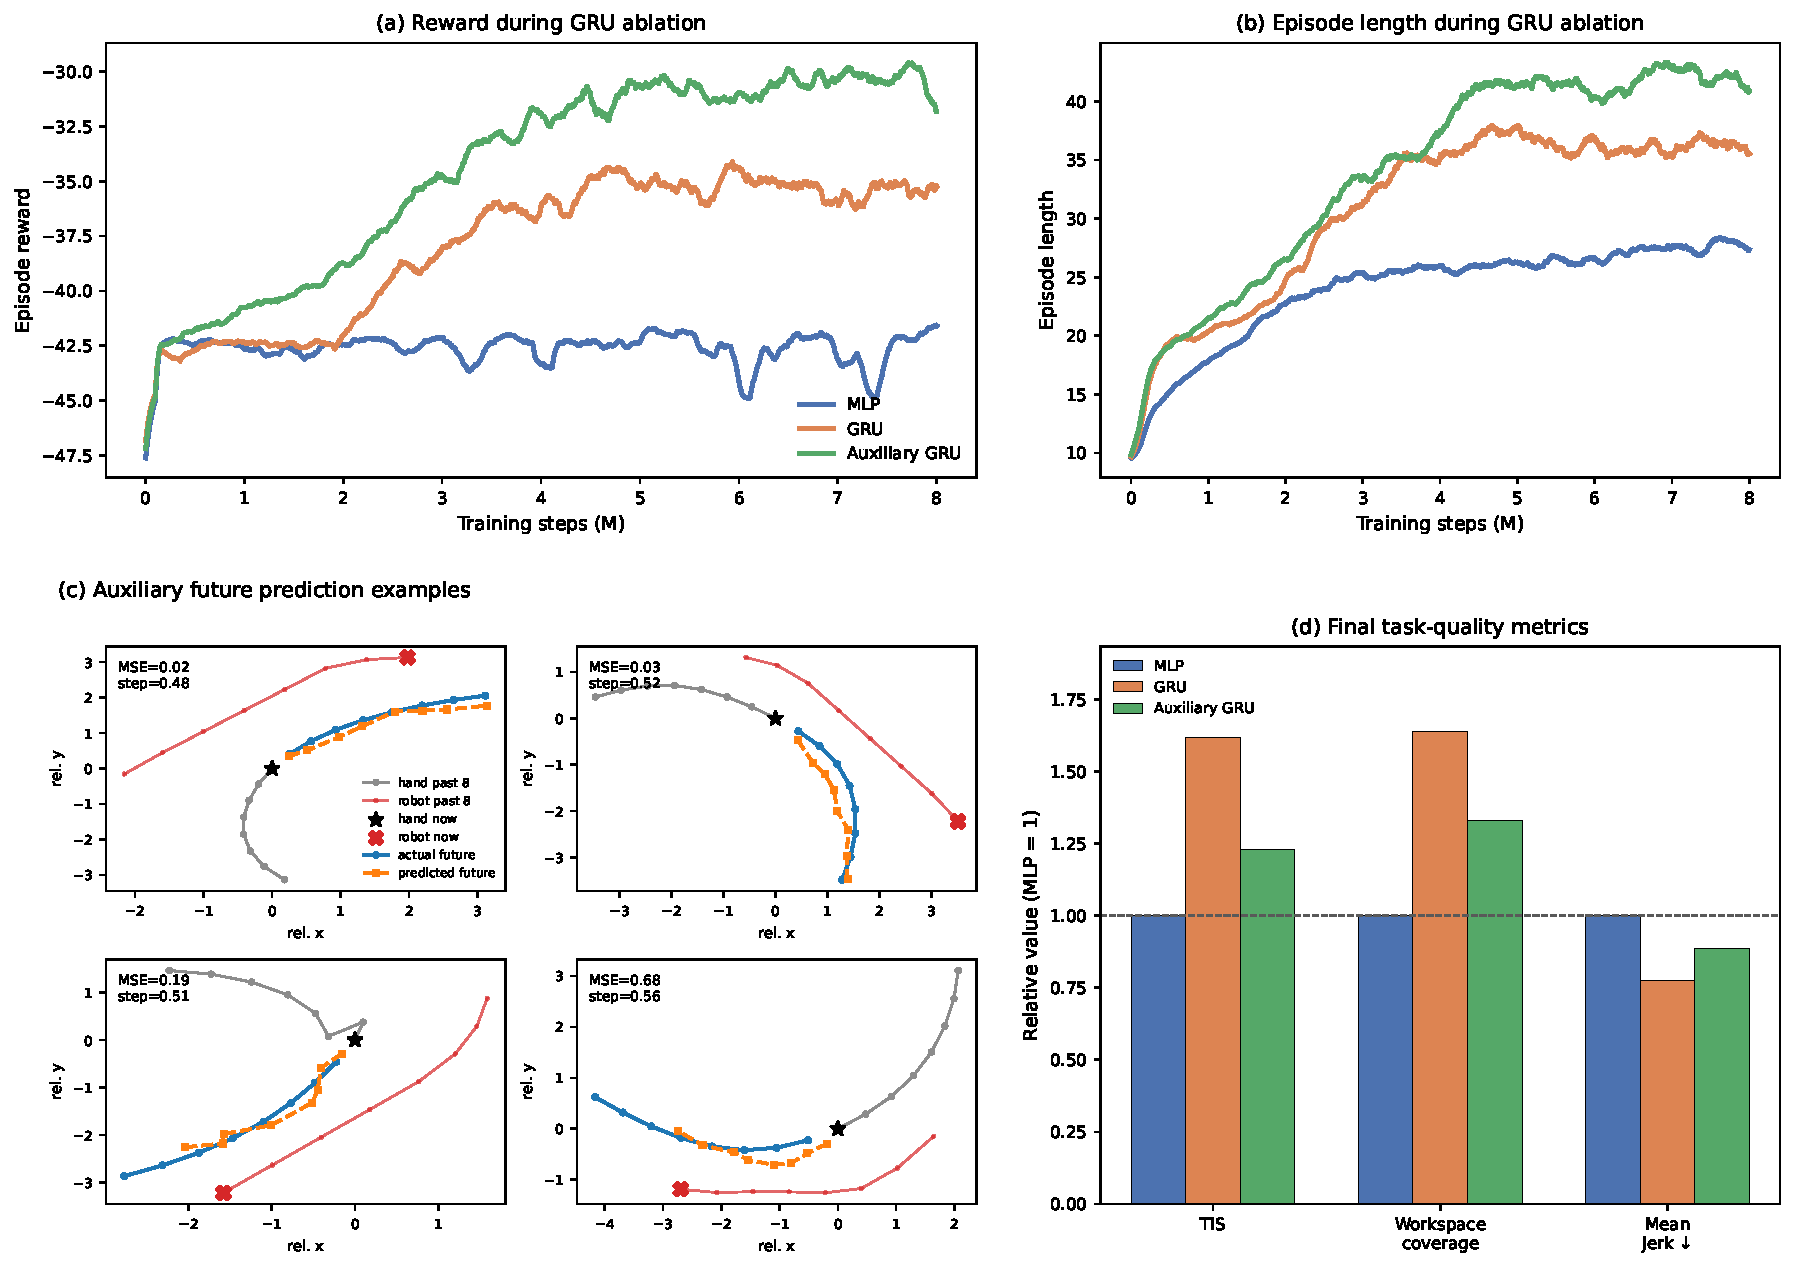
\includegraphics[width=0.98\textwidth]{../manuscripts/figures/paper_ready/fig_sim02_ablation_gru_aux_composite_filled_no_title.png}
\caption{GRU ablation and auxiliary future-motion prediction. Panels (a) and (b) show smoothed raw training reward and episode length for MLP, GRU, and GRU+Aux policies trained against the H1--H10 plus scripted-hand pool. Panels (c) and (d) visualize the auxiliary future-prediction task, showing representative predicted hand trajectories and horizon-dependent trajectory error.}
\label{fig:ablation_composite}
\end{figure*}

\subsection{ZPD and Workspace Metrics}
Table~\ref{tab:ablation_summary} reports the final-stage statistics from the last 10\% of training episodes. Both recurrent variants produce higher ZPD steps and workspace coverage than the MLP baseline. The GRU-only model obtains 22.08 ZPD steps and 0.347 workspace coverage, while GRU+Aux obtains 21.96 ZPD steps and 0.343 workspace coverage. The close values suggest that, under the current weighting and training duration, the auxiliary objective primarily acts as representation supervision rather than producing a clear aggregate-performance advantage over the GRU-only encoder.

\begin{table}[!t]
\caption{Final-stage ablation summary from the last 10\% of training episodes.}
\label{tab:ablation_summary}
\centering
\begin{tabular}{lcccc}
\hline
Method & Reward & Length & ZPD steps & Workspace \\
\hline
MLP & -42.94 & 27.58 & 18.47 & 0.297 \\
GRU & -35.56 & 36.12 & 22.08 & 0.347 \\
GRU+Aux & -35.39 & 35.92 & 21.96 & 0.343 \\
\hline
\end{tabular}
\end{table}

\section{Discussion}
The simulation results suggest two main conclusions. First, league training improves robustness by exposing the robot to a distribution of learned patient behaviors rather than a single scripted controller. The improvement in both mean and worst-case TIS indicates that opponent-pool training can reduce exploitability and better approximate the variability expected across real patients.

Second, temporal interaction history is essential for this task. The gap between the MLP and GRU policies shows that instantaneous spatial state alone is insufficient for reliably adapting to patient behavior. The auxiliary future-prediction task did not yield a large final aggregate advantage over GRU-only training in this run, but it provides a mechanistic and visually interpretable way to verify that the temporal encoder is learning patient-motion dynamics. Future tuning may adjust the auxiliary loss weights, prediction horizon, or curriculum timing to convert this representation benefit into a larger control-performance gain.

These findings support the broader sim-to-real plan. The league-trained robot policy can be transferred to the physical UR10 and magnetic microrobot platform, where asynchronous vision and fixed-rate control will introduce additional latency and noise. Because CMD-DR already randomizes delay, noise, and motor execution, the simulation policy is expected to be more robust to real-world perception-control mismatch than a policy trained against a narrow scripted simulator.

\section{Conclusion}
This draft presented the simulation-stage evidence for an adaptive RL framework for upper-limb rehabilitation. A ten-generation league improved both mean and worst-case ZPD time-in-zone against learned hand opponents. A GRU ablation showed that recurrent interaction-history encoding substantially improves reward, episode length, ZPD steps, and workspace coverage relative to an MLP baseline. The auxiliary future-prediction head offers interpretable supervision for latent patient-dynamics inference, even though its aggregate control advantage over GRU-only training remains modest in the current run. The next stage is to integrate these simulation results with the real-world vision-control architecture and physical UR10 validation.

\balance

\begin{thebibliography}{1}

\bibitem{placeholder_rl_rehab}
Reference list to be completed with rehabilitation robotics, reinforcement learning, self-play, domain randomization, and sim-to-real transfer literature.

\end{thebibliography}

\end{document}
